\ylDisplay
{}% Problem name
{2021}% Year
{mcq}% Round (mcq, theory, experiment)
{8}% Problem nr.
{physics}% Subject (physics, chemistry, biology)
{}% Difficulty (1-3)
{
% Syl:
\ifStatement
While doing an experiment in physics laboratory, Mustafa connected two coils (say coil $B$ and coil $A$) in series with a galvanometer and dropped a magnet through the coils, as shown in the figure. He noticed that there was no deflection in the galvanometer when the magnet passed through coil $A$ and observed a large deflection when it passed through coil $B$. He noticed that both coils are identical in shape, size and material. Both had same number of turns and the speed with which the magnet passed through each coil was nearly the same. He correctly concluded that
\begin{figure}[!htbp]
  \centering
  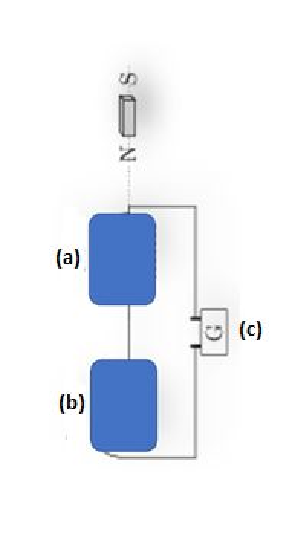
\includegraphics[width=.2\linewidth]{2021-mcq-08-p}
  \caption{(a) Coil A (b) Coil B (c) Galvanometer}
\end{figure}
\fi


\ifOption1
The net magnetic flux through coil A must be zero.
\fi


\ifOption2
When passing through coil A, induced emf across coils B and A must be in the opposite directions.
\fi


\ifOption3
The galvanometer would show deflection for coil A if the poles of the bar magnet were reversed.
\fi


\ifOption4
Coil A must have different pattern of windings than that of coil B.
\fi


\ifHint

\fi


\ifSolution

\fi


\ifEstStatement
% Problem name:

\fi


\ifEstOption1

\fi


\ifEstOption2

\fi


\ifEstOption3

\fi


\ifEstOption4

\fi


\ifEstHint

\fi


\ifEstSolution

\fi
}
